\documentclass{article}

\usepackage[utf8]{inputenc}
\usepackage{polski}
\selecthyphenation{polish}
\usepackage{verbatim}
\usepackage{graphicx}
\usepackage{amssymb}
\usepackage{amsmath}
\usepackage{hyperref}
\usepackage{multirow}

% do \makegapedcells
\usepackage{makecell}
\setcellgapes{4pt}


\usepackage{makeidx}
\makeindex

\title{Projekt  \LaTeX}
\author{Michał Kocisz}
\date{\today}

\begin{document}

\maketitle
\tableofcontents
\listoftables
\pagebreak

\section{Wprowadzenie}
\subsection{Fizyka - definicja}

\textbf{Fizyka} (\textit{„natura”}) – nauka przyrodnicza zajmująca się badaniem najbardziej fundamentalnych i uniwersalnych właściwości oraz przemian materii i energii, a także oddziaływań między nimi. Do opisu zjawisk fizycznych fizycy używają wielkości fizycznych, wyrażonych za pomocą pojęć matematycznych, takich jak liczba, wektor, tensor. Tworząc hipotezy i teorie fizyki, budują relacje pomiędzy wielkościami fizycznymi.

Z fizyką ściśle wiążą się inne nauki przyrodnicze, szczególnie chemia. Chemicy przyjmują teorie fizyki dotyczące cząsteczek i związków chemicznych (mechanika kwantowa, termodynamika) i za ich pomocą tworzą teorie w ich własnych dziedzinach badań. Fizyka zajmuje szczególne miejsce w naukach przyrodniczych, ponieważ wyjaśnia podstawowe zależności obowiązujące w przyrodzie.

\subsection{Działy fizyki}

\begin{table}[h]
\centering
\index{tabele!Główne teorie}
  \caption[Główne teorie]{
    \label{fiztab1}
    Główne teorie \vspace{2ex}
  }
\vspace{2ex}
  \centering
 \begin{tabular}{| l | l |}
	\hline
    \textbf{Teoria} & \textbf{Działy}\\ \hline
mechanika klasyczna &\vtop{\hbox{\strut  zasady dynamiki Newtona, teoria chaosu, }\hbox{\strut mechanika płynów}} \\ \hline
termodynamika i mechanika statystyczna & kinetyczno-molekularna teoria gazów \\ \hline
elektrodynamika klasyczna & \vtop{\hbox{\strut  elektrostatyka, elektryczność, magnetyzm, }\hbox{\strut równania Maxwella}}  \\ \hline
teoria względności &  \vtop{\hbox{\strut szczególna teoria względności, }\hbox{\strut  ogólna teoria względności}}  \\ \hline
mechanika kwantowa &  \vtop{\hbox{\strut równanie Schrödingera, kwantowa teoria pola,  }\hbox{\strut elektrodynamika kwantowa,}\hbox{\strut chromodynamika kwantowa}}  \\ \hline
  \end{tabular}  
\end{table}

\pagebreak
\index{tabele!Działy szczegółowe fizyki}
\begin{table}[h]
\centering
  \caption[Działy szczegółowe fizyki]{
    \label{fiztab2}
    Działy szczegółowe fizyki \vspace{2ex}
  }
\vspace{2ex}
  \centering
 \begin{tabular}{| l | l | l |}
	\hline
    \textbf{Działy} & \textbf{Poddziały} & \textbf{Główne teorie}\\ \hline

astrofizyka &\vtop{\hbox{\strut kosmologia, nauki planetarne, }\hbox{\strut fizyka plazmy}}  &\vtop{\hbox{\strut ogólna teoria względności, }\hbox{\strut  Wielki Wybuch,}\hbox{\strut inflacja kosmologiczna}} \\ \hline

\vtop{\hbox{\strut fizyka atomów, cząsteczek }\hbox{\strut i zjawisk optycznych}} &\vtop{\hbox{\strut	fizyka atomowa, optyka, }\hbox{\strut  fotonika}}  & optyka kwantowa\\ \hline

fizyka cząstek elementarnych &fizyka jądrowa  &\vtop{\hbox{\strut model standardowy, teorie}\hbox{\strut wielkiej}\hbox{\strut unifikacji, teoria superstrun,}\hbox{\strut  M-teoria}} \\ \hline

fizyka fazy skondensowanej &\vtop{\hbox{\strut fizyka ciała stałego, fizyka }\hbox{\strut polimerów, fizyka niskich}\hbox{\strut temperatur}}  & gaz Fermiego, teoria BCS \\ \hline
  \end{tabular}  
\end{table}

\section{Grawitacja}

\subsection{Prawo powszechnego ciążenia}

\textbf{Prawo powszechnego ciążenia}, zwane także prawem powszechnego ciążenia Newtona, głosi, że każdy obiekt we wszechświecie przyciąga każdy inny obiekt z siłą, która jest wprost proporcjonalna do iloczynu ich mas i odwrotnie proporcjonalna do kwadratu odległości między ich środkami. Jest to ogólne prawo fizyczne, bazujące na empirycznych obserwacjach Newtona, które nazwał on indukcją (wpływem)\index{grawitacja!Newton|textbf}. Wchodzi ono w skład podstaw mechaniki klasycznej i zostało sformułowane w pracy sir Isaaca Newtona pt.: \textit{Philosophiae naturalis principia mathematica}~\cite{NEW87}, opublikowanej po raz pierwszy 5 lipca 1687 r. 
\noindent
\framebox[4cm][r]{Zobacz mechanizm: ~\ref{rys:newton-picture}.}

\paragraph{Matematycznie związek ten wyraża się wzorem:\index{grawitacja!Wzór powszechnego ciążenia}}

\begin{equation}
  \mathrm{F}^{i}= \mathrm{G}\frac{\mathrm{m}_{1}\mathrm{m}_{2}}{\mathrm{r}^{2}}\mathrm{e}^{i}
\end{equation}
\paragraph{Stała grawitacji została uznana za jedną z podstawowych stałych fizycznych. Z pomiarów wynika, że jej wartość wynosi:\index{grawitacja!Stała grawitacji}}
\begin{equation}
{\displaystyle G\approx 6,6732(\pm 0,0031)10^{-11}\operatorname {m} ^{3}\operatorname {kg} ^{-1}\operatorname {s} ^{-2}.}
\end{equation}\\[2ex]

\begin{figure}[h]
\caption{\label{rys:newton-picture}
    Mechanizmy prawa powszechnego ciążenia Newtona.
  }
  \centering
   \setlength{\unitlength}{1 cm}
    \begin{picture}(10,5)(0,0)

      \put(2.5, 2.5){\circle{4}}
      \put(2.2, 2.5){  ${m}_{1}$}
      \put(3.2,2.5){\vector(1,0){1}}
      \put(3.3, 2.7){  ${F}_{1}$}
      \put(7.5, 2.5){\circle{1}}
      \put(7.2, 2.5){  ${m}_{2}$}
      \put(7,2.5){\vector(-1,0){1}}
      \put(6.4, 2.7){  ${F}_{2}$}

      \put(2.5,1.8){\line(0,-1){1}}
      \put(7.5,2){\line(0,-1){1.2}}
      \put(2.5,1){\vector(1,0){5}}
      \put(7.5,1){\vector(-1,0){5}}

      \put(5, 1.1){ r}

    \end{picture}
\end{figure}

\subsection{Prawa Keplera ruchu planet}

Johannes Kepler wnikliwie przeanalizował dane dotyczące ruchu planet uzyskane przez Tychona de Brahe. Na tej podstawie wykazał, że planety poruszają się według określonych praw zgodnych z teorią Kopernika; prawa te umożliwiły Newtonowi odkrycie prawa powszechnego ciążenia. Rezultaty tych prac opublikował w roku 1609 w dziele \textit{Astronomia Nova}~\cite{KEP09}.

Kepler stwierdził, że ruchem planet rządzą trzy proste prawa (prawa Keplera stosują się również do ruchu satelitów okrążających dowolną planetę).

\paragraph{Pierwsze prawo Keplera:\index{grawitacja!1 prawo Keplera}}

\begin{center}
\textsl{Każda planeta krąży po orbicie eliptycznej, a Słońce znajduje się w jednym z dwóch ognisk elipsy.}
\end{center}

\paragraph{Drugie prawo Keplera:\index{grawitacja!2 prawo Keplera}}

\begin{center}
\textsl{Promień wodzący poprowadzony ze środka Słońca do środka planety zakreśla równe pola powierzchni w równych odstępach czasu.}
\end{center}
\noindent
\framebox[4cm][r]{Zobacz obrazek: ~\ref{rys:kepler2}.}

\paragraph{Trzecie prawo Keplera:\index{grawitacja!3 prawo Keplera}}

\begin{center}
\textsl{Sześciany wielkich półosi orbit jakichkolwiek dwóch planet mają się tak do siebie, jak kwadraty ich okresów obiegu. W przypadku orbit kołowych (okrąg jest szczególnym przypadkiem elipsy):}

\begin{equation}
  \frac{\mathrm{r}_{1}^{3}}{\mathrm{r}_{2}^{3}} = \frac{\mathrm{T}_{1}^{2}}{\mathrm{T}_{2}^{2}}
\end{equation}
\end{center}
\index{wzory!3 prawo Keplera}
\pagebreak

\begin{figure}[h]
\centering
\caption[2 prawo Keplera obrazek]{\label{rys:kepler2}
    Graficzna interpretacja II Prawa Keplera
} \vspace{2ex}
 \framebox{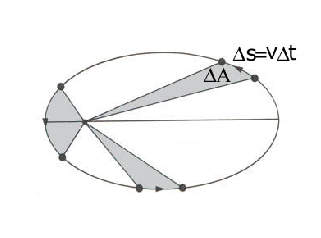
\includegraphics[width=0.6\textwidth]{img1.eps}}
\end{figure}
\index{Planety!{Interpretacja drugiego prawa Keplera}}

\section{Termodynamika}
\subsection{Przemiana izochoryczna}

\textbf{Przemiana izochoryczna} – proces termodynamiczny zachodzący przy stałej objętości $(V = const)$. Oprócz objętości wszystkie pozostałe parametry termodynamiczne mogą się zmieniać.
\index{termodynamika!przemiana izochoryczna|textbf}
Podczas przemiany izochorycznej nie jest wykonywana praca, układ może wymieniać energię z otoczeniem tylko w wyniku cieplnego przepływu energii. Z pierwszej zasady termodynamiki wynika, że całe ciepło doprowadzone lub odprowadzone z gazu w procesie izochorycznym jest zużywane na powiększenie lub pomniejszenie jego energii wewnętrznej: ${\displaystyle \delta Q={\text{d}}U}$.
\vspace{2ex}

Przekształcając wzór na ciepło właściwe otrzymujemy:
\begin{equation}
{\displaystyle {\text{d}}U=c_{V}mdT,}
\end{equation}
\index{wzory!przemiana izochoryczna}
gdzie:

${\displaystyle m}$  – masa gazu.
\vspace{2ex}

W przypadku gazu doskonałego wzór ten jest słuszny dla dowolnego procesu, natomiast dla gazu rzeczywistego wzór ten jest słuszny tylko w zakresie niewielkich zmian temperatur. Przy większych zmianach ciepło właściwe $cV$ gazu rzeczywistego nie może być traktowane jako stała. ~\cite{LPVS05}
\vspace{2ex}

Zmianę energii wewnętrznej można obliczyć w następujący sposób:
\begin{equation}
{\displaystyle \Delta U=\int \limits _{T_{1}}^{T_{2}}{c_{V}mdT}=c_{V}m(T_{2}-T_{1})=c_{V}m\Delta T,} 
\end{equation}
\index{wzory!zamiana energii wew. przemiany izochorycznej}
gdzie:

${\displaystyle c_{V}}$ – ciepło właściwe w procesie izochorycznym.
\vspace{2ex}

Proces izochoryczny można praktycznie zrealizować podczas ogrzewania lub oziębiania gazu w zbiorniku o stałej objętości, czyli wykonanego z materiału o zerowej rozszerzalności cieplnej.

\begin{figure}[h]
\centering
\caption[Przemiana izochoryczna]{\label{rys:termo}
    Izochory wody i pary wodnej na wykresie h-s (entalpia-entropia), czarnym kolorem naniesiona jest linia nasycenia, czerwonym – linie stałego stopnia suchości pary
} \vspace{2ex}
 \framebox{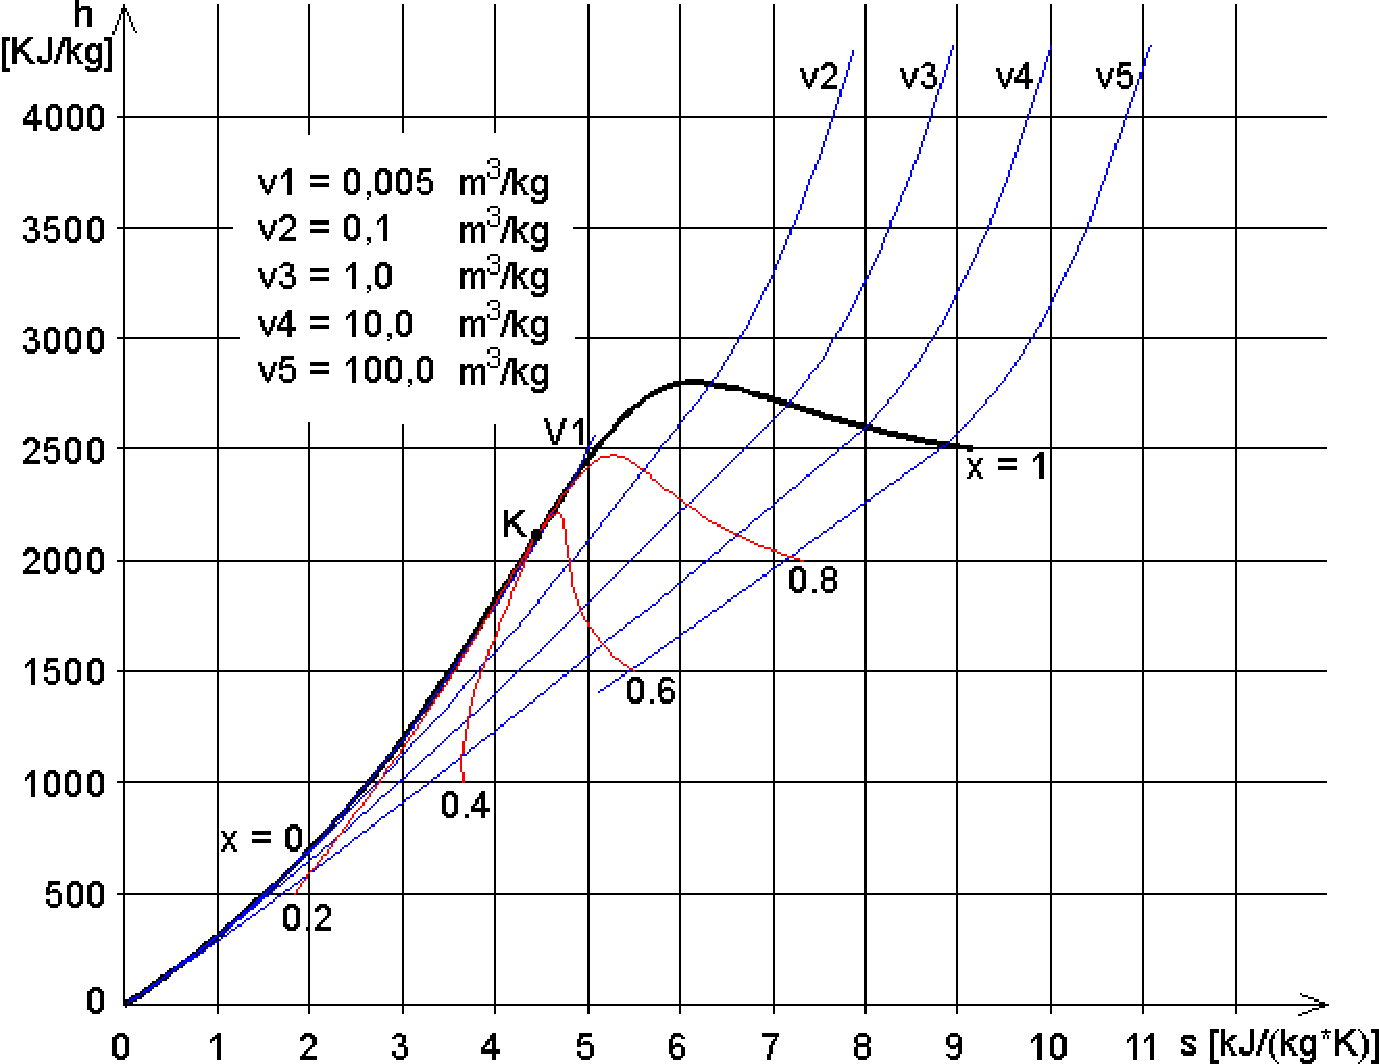
\includegraphics[width=0.9\textwidth]{img2.pdf}}
\end{figure}
\index{Izochory!{Izochory wody i pary wodnej na wykresie}}

\subsection{Przemiana izobaryczna}
\index{termodynamika!Przemiana izobarycznan|textbf}
\textbf{Przemiana izobaryczna} – proces termodynamiczny, podczas którego ciśnienie układu nie ulega zmianie, natomiast pozostałe parametry termodynamiczne czynnika mogą się zmieniać. Procesy izobaryczne mogą zachodzić zarówno w sposób odwracalny, jak i nieodwracalny. Odwracalny proces izobaryczny przedstawia na wykresie krzywa zwana izobarą. Praca wykonana przez układ (lub nad układem) w odwracalnym procesie izobarycznym jest równa ubytkowi (lub przyrostowi) entalpii układu. W szczególności, gdy jedyny wkład do pracy stanowi praca objętościowa (polegająca na zmianie objętości układu), jest ona wyrażona wzorem:
\begin{equation}
{\displaystyle W=p\Delta V,} 
\end{equation}
\index{wzory!praca objętościowa w przem. izobarycznej}
gdzie:
\vspace{2ex}

${\displaystyle W}$ – praca wykonana przez układ,
\vspace{2ex}

${\displaystyle p}$ – ciśnienie,
\vspace{2ex}

${\displaystyle \Delta V}$ – wzrost objętości układu.
\vspace{2ex}

Dla gazu doskonałego przemiana izobaryczna spełnia zależność 
\begin{equation}
{\displaystyle {\frac {V}{T}}=\operatorname {const} ,}
\end{equation}
\index{wzory!{zależność gazu doskonałego w przem. izobarycznej}}
gdzie:
\vspace{2ex}

${\displaystyle V}$ – objętość,
\vspace{2ex}

${\displaystyle T}$ – temperatura.

\begin{figure}[h]
\centering
\caption[Przemiana izobaryczna]{\label{rys:termo2}
   Na poniższych rysunkach przedstawione są przemiany izobaryczne wody i pary wodnej w układzie$ h-s$ (entalpia właściwa – entropia właściwa) i $T-s$ (temperatura – entropia właściwa) na tle linii nasycenia i stałego stopnia suchości pary.
} \vspace{2ex}
 \framebox{
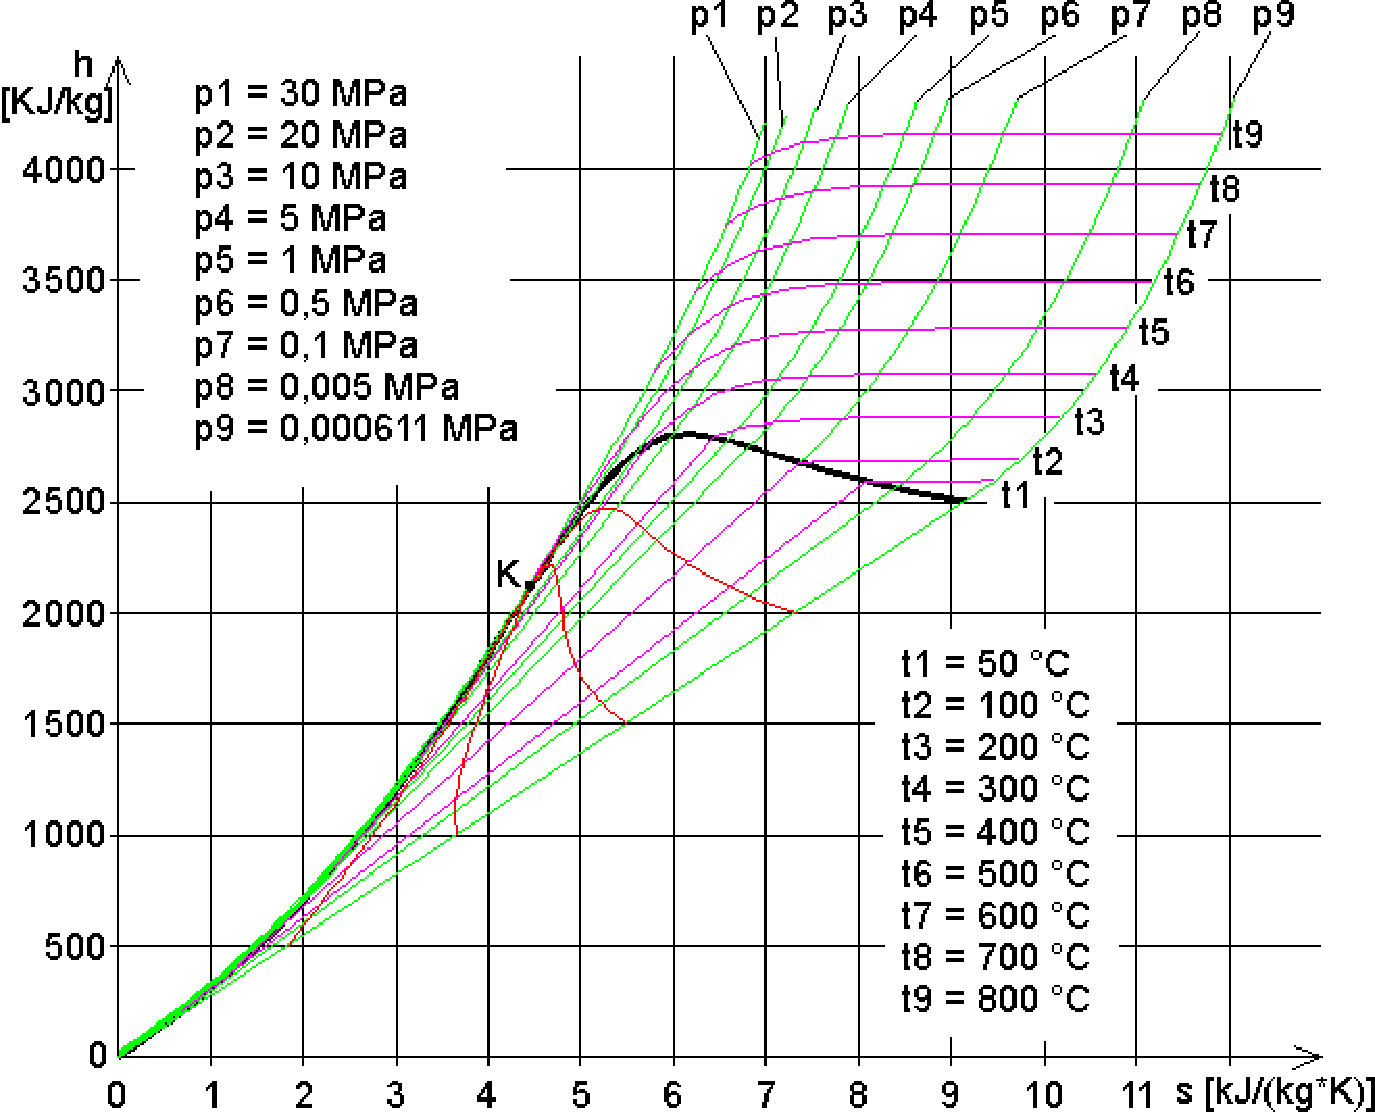
\includegraphics[width=0.5\textwidth]{img3.pdf}
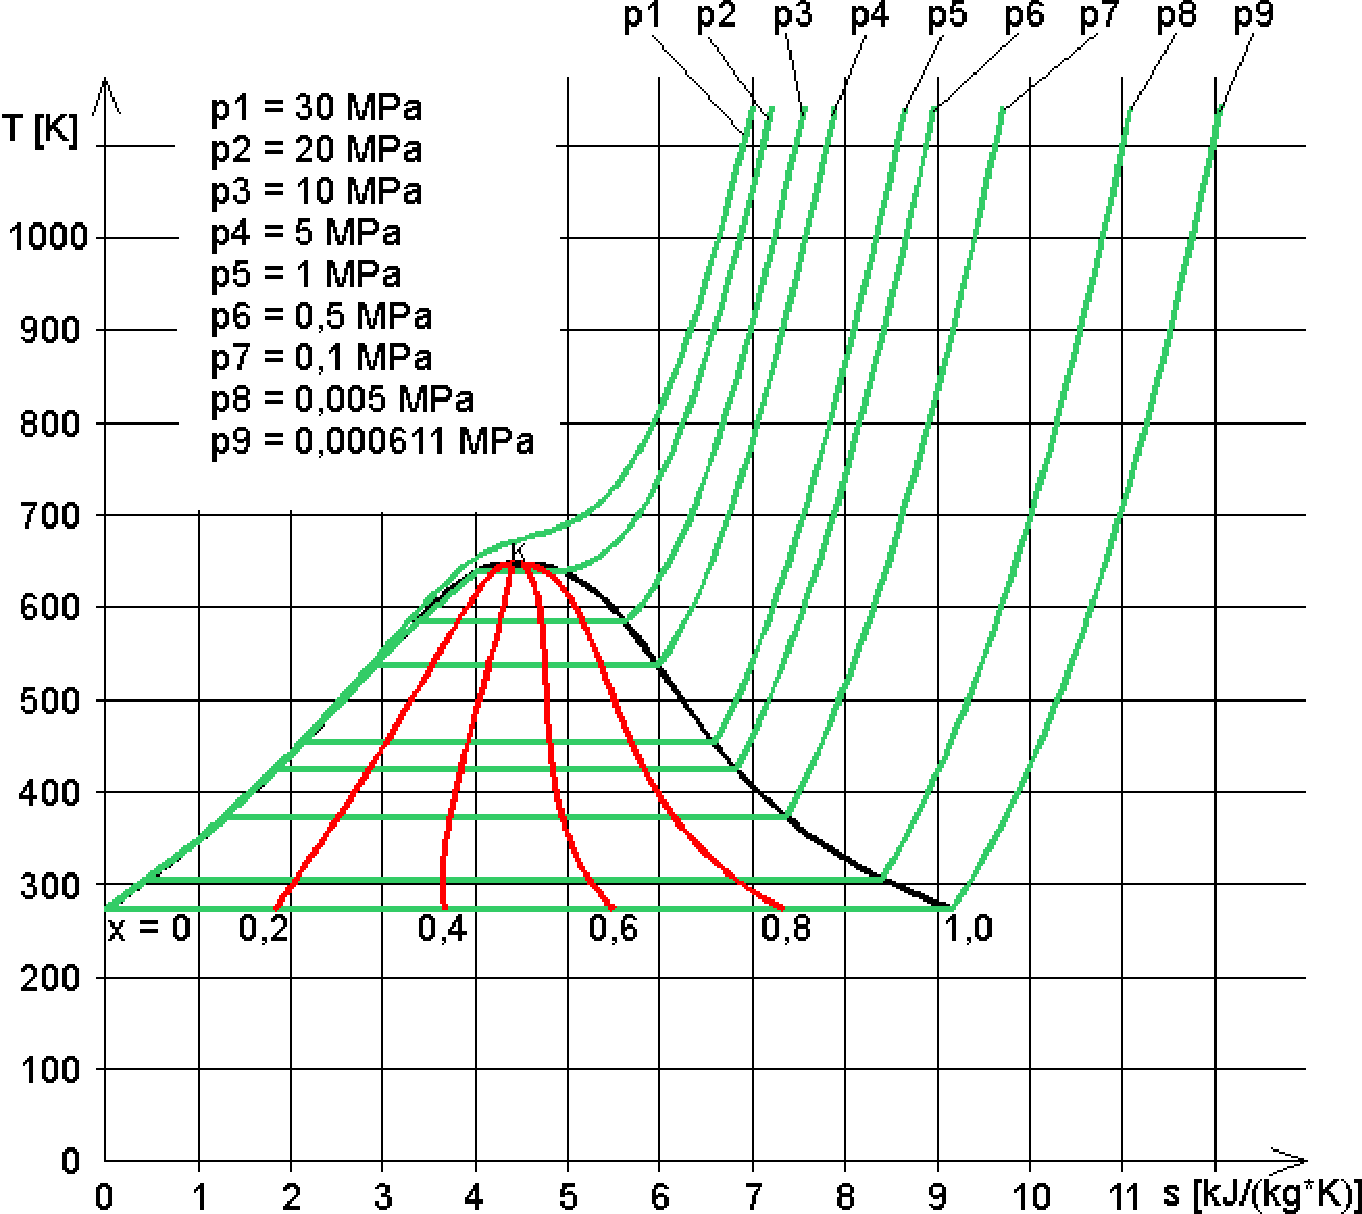
\includegraphics[width=0.5\textwidth]{img4.pdf}
}
\end{figure}
\index{Izobary!{Przemiany izobaryczne wody i pary wodnej}}

\pagebreak

\subsection{Przemiana izotermiczna}

\textbf{Przemiana izotermiczna} – w termodynamice przemiana, zachodząca przy określonej, stałej temperaturze. Krzywa opisująca przemianę izotermiczną nazywana jest izotermą. ~\index{termodynamika!Przemiana izotermiczna|textbf}
\vspace{2ex}

\textbf{Przemiana izotermiczna gazu doskonałego}
~\index{termodynamika!gaz doskonały}
Dla gazu doskonałego, energia wewnętrzna jest funkcją temperatury. Dlatego w przemianie izotermicznej, ponieważ ${\displaystyle \Delta T=0}$, zachodzi zależność:
\begin{equation}
{\displaystyle \Delta U=nR\Delta T=0,}
\end{equation}

co wyrażane jest też prawidłowością:
\begin{equation}
{\displaystyle \Delta (pV)=0}
\end{equation}
\hspace{5ex}lub
\begin{equation}
{\displaystyle p_{i}V_{i}=pV=p_{f}V_{f}}
\end{equation}
\hspace{5ex}lub
\begin{equation}
{\displaystyle pV=\mathrm {const} ,}
\end{equation}
\index{wzory!{Wzór przemiany izotermicznej}}
gdzie:
\vspace{2ex}

${\displaystyle p_{i}}$  i  ${\displaystyle V_{i}}$ – ciśnienie i objętość początkowa,
\vspace{2ex}

${\displaystyle p_{f}}$ i ${\displaystyle V_{f}}$ – ciśnienie i objętość końcowa,
\vspace{2ex}

${\displaystyle p}$  i ${\displaystyle V}$ – zmienne opisujące zachowanie się gazu podczas przemiany izotermicznej.
\vspace{2ex}

 Powyższa zależność między ciśnieniem i objętością dla gazu doskonałego stanowi treść prawa \href{https://pl.wikipedia.org/wiki/Prawo_Boyle%E2%80%99a-Mariotte%E2%80%99a}{\textbf{Boyle’a-Mariotte’a}}.~\index{prawo Boyle’a-Mariotte’a}
\vspace{2ex}

Izoterma gazu doskonałego jest hiperbolą na wykresie $p-V$ (ciśnienie-objętość) ($T = constant$)
\begin{equation}
{\displaystyle p={\frac {nRT}{V}}.}
\end{equation}


Z \href{https://pl.wikipedia.org/wiki/Pierwsza_zasada_termodynamiki}{pierwszej zasady termodynamiki} wynika, że całe ciepło doprowadzone do gazu doskonałego w procesie izotermicznym jest zużywane na wykonanie pracy przeciwko siłom zewnętrznym.
\begin{equation}
{\displaystyle Q=W.}
\end{equation}
Załóżmy, że mamy gaz w zbiorniku, zamknięty ruchomym tłokiem o polu powierzchni $S$. Dla bardzo małego przesunięcia tłoka $dx$ praca $dW$ może być zapisana wzorem:
\begin{equation}
{\displaystyle \mathrm {d} W=F\,\mathrm {d} x=pS\,\mathrm {d} x=p\,\mathrm {d} V.}
\end{equation}
Praca, jaką wykonuje gaz, rozszerzając się od objętości ${\displaystyle V_{A}}$ do ${\displaystyle V_{B}}$, wyraża wzór:
\begin{equation}
{\displaystyle W_{A\to B}=\int \limits _{V_{A}}^{V_{B}}\mathrm {d} W=\int \limits _{V_{A}}^{V_{B}}p\,\mathrm {d} V} 
\end{equation}
w procesie izotermicznym
\begin{equation}
{\displaystyle W_{A\to B}=\int \limits _{V_{A}}^{V_{B}}p\,\mathrm {d} V=\int \limits _{V_{A}}^{V_{B}}{\frac {nRT}{V}}\mathrm {d} V=nRT\ln {\frac {V_{B}}{V_{A}}}=nRT\ln {\frac {P_{A}}{P_{B}}}.}
\end{equation}
\vspace{2ex}

Proces izotermiczny jest jedną z przemian w cyklu Carnota,
\vspace{2ex}

gdzie:
\vspace{2ex}
\begin{itemize}
\item $W$ – praca wykonana przez gaz,
\item $Q$ – ciepło doprowadzone,
\item $p$ – ciśnienie,
\item $V$ – objętość,
\item $n$ – liczba moli gazu,
\item $R$ – uniwersalna stała gazowa.
\end{itemize}

\pagebreak

\subsection{Ciecze}

\begin{table}[h]
\makegapedcells % żeby ładnie zrobić odstępy pionowo, wymaga dodatkowego pakietu
\centering
\index{tabele!Ciecze}
  \caption[Tabela cieczy]{
    \label{fiztab3}
    Ciecze \vspace{2ex}
  }
\vspace{2ex}
  \centering
 \begin{tabular}{|| c | c | c ||}
	\hline \hline
    \textbf{Wielkość} & \textbf{Wzór} & \textbf{Jednostka} \\[2pt] \hline
ciepło parowania & ${\displaystyle C_{p}=\frac{Q}{m}}$ &  ${\displaystyle 1\frac{J}{kg}}$ \\[2pt] \hline

ciśnienie kapilarne & ${\displaystyle p=\frac{2\delta}{r}}$ &   \\[2pt] \hline

prawo wzniesienia kapilarnego & ${\displaystyle h=\frac{2\delta}{r({D}_{1}-{D}_{2})g}}$ &  \\[2pt] \hline

\multirow{2}{*}{napięcie powierzchniowe $\delta$} & ${\displaystyle \delta=\frac{W}{\Delta S}}$ &  ${\displaystyle 1\frac{J}{{m}^{2}}}$ \\ &  ${\displaystyle \delta=\frac{F}{I}}$ &  ${\displaystyle 1\frac{N}{m}}$ \\[2pt] \hline

współczynnik lepkości $\eta$ & ${\displaystyle \eta=\frac{F}{US}}\ i\ {\displaystyle U=\frac{dv}{dz}}$ &  ${\displaystyle 1\frac{kg}{ms}}$ \\[2pt] \hline\hline
  \end{tabular}  
\end{table}

\printindex
\bibliographystyle{alpha}
\bibliography{bib}
\listoffigures

\end{document}


























